\documentclass[./thesis.tex]{subfiles}

\begin{document}

In this chapter, we discuss the efficiency of the implementation. The system
we chose for these numerical experiments is a cyanine dye,
[(NH$_2$)(CH)(NH$_2$)]$^+$ in its ground state and in its first excited state.
The geometry is the equilibrium geometry of the ground state, optimized at the
PBE0/cc-pVQZ level. The ground state is a closed shell, well described by a
single reference, and the excited state is singly excited and requires two
determinants in the reference ($1/\sqrt{2} (a\bar{b} + b\bar{a})$).  The
calculations were performed in the aug-cc-pVDZ basis set with state-averaged
natural orbitals obtained from an initial CIPSI calculation.
The $1s$ orbitals of the carbon and the nitrogen atoms were frozen, so
the FCI space which is explored is a CAS(18,111). The reference excitation
energy, obtained at the CC3/ANO-L-VQZP level is 7.18~eV\cite{Send_2011}.


\section{Davdison diagonalization}

\begin{table}
\caption{Time (in seconds) to run one Davidson's iteration in parallel on the largest wave function
with an increasing number of 36-core compute nodes.}
\label{tab:energy_pt2}
\begin{center}
\begin{tabular}{rr}
\hline
\tabc{Nodes} & \tabc{Wall-clock time (s)} \\
\hline
$ 1$ &$12~361.68$ \\
$ 5$ &$ 2~580.70$ \\
$10$ &$ 1~363.24$ \\
$20$ &$   746.36$ \\
$30$ &$   542.91$ \\
$40$ &$   442.11$ \\
$50$ &$   381.92$ \\
\hline
\end{tabular}
\end{center}
\end{table}


\section{Selection}


\section{PT2 calculations}

The stopping criterion of the calculation of the PT2 contribution was a
relative statistical error below 1/1000-th.
The fraction of the full deterministic calculation required to reach this criterion
is typically around $5\%$.
The measurements were made on the Olympe supercomputer (CALMIP). Each node is 
a dual-socket Intel(R) Xeon(R) Gold 6140 CPU @ 2.30GHz with 192GiB of RAM, and
contains 36 physical CPU cores.

\begin{figure}[h]
	\begin{center}
		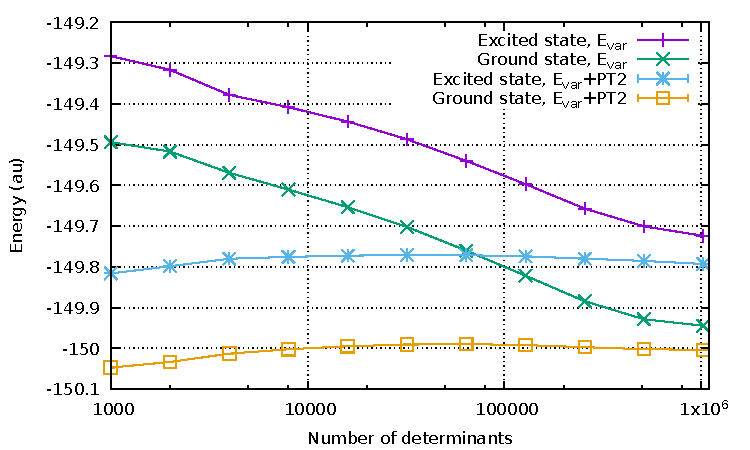
\includegraphics[width=0.8\columnwidth]{figures/pt2/cn3_energy}
		\caption{Convergence of the energy of the ground and excited states with respect to the number of determinants in the variational space.}
		\label{fig:energy_pt2}
	\end{center}
\end{figure}
\begin{figure}[h]
	\begin{center}
		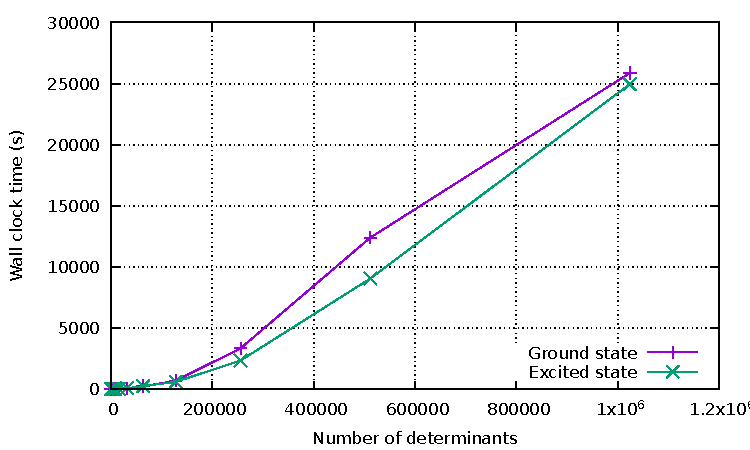
\includegraphics[width=0.8\columnwidth]{figures/pt2/scaling_det}
		\caption{Wall clock time required to compute the PT2 contribution for the ground and the excited states, as a function of the number of determinants in the wave function.}
		\label{fig:scaling_det_pt2}
	\end{center}
\end{figure}

\begin{table}
\caption{Single-node (36-core) $\EPT$ calculations for increasingly large wave functions. Time is given in seconds, and energies are given in atomic units.}
\label{tab:energy_pt2}
\begin{center}
\begin{tabular}{rllr}
\hline
\tabc{$\Ndet$} & \tabc{$\Evar$} & \tabc{$\EPT$} & \tabc{Time} \\
\hline
\multicolumn{4}{c}{Ground state}  \\
$      7$ & $-149.489~186$ & $-150.161~107  $ & $    0.00$ \\
$    123$ & $-149.536~265$ & $-150.116~958  $ & $    0.48$ \\
$   3083$ & $-149.685~606$ & $-150.043~5(2) $ & $    1.53$ \\
$  29409$ & $-149.826~151$ & $-150.022~2(2) $ & $   13.71$ \\
$ 168595$ & $-149.900~352$ & $-150.019~9(1) $ & $  138.17$ \\
$1322537$ & $-149.946~655$ & $-150.017~89(7)$ & $ 2456.66$ \\
$8495334$ & $-149.972~032$ & $-150.015~97(4)$ & $38350.47$ \\
$9356952$ & $-149.973~375$ & $-150.015~95(4)$ & $44873.53$ \\
\hline
\multicolumn{4}{c}{Excited state} \\
$      7$ & $-149.207~354$ & $-149.904~883  $ $    0.00$ \\
$    123$ & $-149.261~860$ & $-149.849~465  $ $    0.53$ \\
$   3083$ & $-149.404~450$ & $-149.780~8(2) $ $    2.05$ \\
$  29409$ & $-149.547~275$ & $-149.758~3(2) $ $   23.75$ \\
$ 168595$ & $-149.626~058$ & $-149.754~5(1) $ $  155.36$ \\
$1322537$ & $-149.675~032$ & $-149.752~55(7)$ $ 2640.67$ \\
$8495334$ & $-149.704~145$ & $-149.750~87(5)$ $42796.15$ \\
$9356952$ & $-149.706~822$ & $-149.750~68(4)$ $50361.70$ \\
\hline
\end{tabular}
\end{center}
\end{table}

\begin{table}
\caption{Time (in seconds) to run parallel $\EPT$ calculations on the largest wave function with an
increasing number of 36-core compute nodes.}
\label{tab:energy_pt2}
\begin{center}
\begin{tabular}{rrr}
\hline
\tabc{Nodes} & \tabc{Ground state} & \tabc{Excited state} \\
\hline
$ 1$ & $44~873.53$ & $50~361.70$ \\
$ 5$ & $10~552.02$ & $11~260.12$ \\
$10$ & $ 5~381.51$ & $ 5~918.34$ \\
$20$ & $ 2~782.87$ & $ 3~043.94$ \\
$30$ & $ 1~884.67$ & $ 2~069.17$ \\
$40$ & $ 1~440.96$ & $ 1~568.30$ \\
$50$ & $ 1~154.97$ & $ 1~273.66$ \\
\hline
\end{tabular}
\end{center}
\end{table}

In figure~\ref{fig:energy_pt2}, we plot the convergence of the energies of
the ground and excited states as a function of the number of
determinants, with and without the second order perturbative contribution.
Table~\ref{tab:energy_pt2} reports the corresponding values, as well as the
wall-clock time required to compute the PT2 contribution on a single node.

From these data, one can evaluate the scaling of the cost of the PT2 contribution
with the number of determinants, as plotted in figure~\ref{fig:scaling_det_pt2}.
We first remark an $\order{N^2}$-like behavior for small sizes, which is consistent
with the fact that
\begin{enumerate}
\item the number of $\ket{\alpha}$ determinants is proportional to the
number of generators, and 
\item each $\ket{\alpha}$ needs to be compared to all the determinants of the wave function in the computation of $\mel{\alpha}{H}{\Psi}$.
\end{enumerate}
But when the wave function becomes large enough, the second point is not true any more because only a limited number of determinants $\ket{I}$ of $\Psi$ have a non-zero
value $\mel{\alpha}{H}{I}$, and this number is bounded by the number of single and double excitations, characteristic of the basis set. This explains the asymptotic linear scaling behavior one can observe.
\begin{figure}[h]
	\begin{center}
		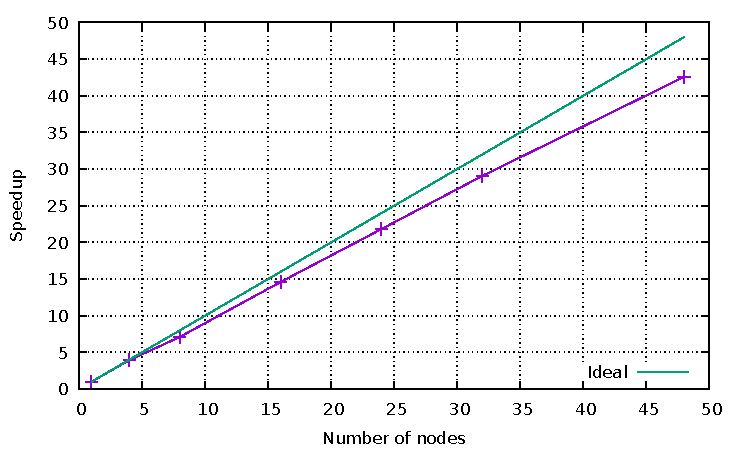
\includegraphics[width=0.8\columnwidth]{figures/pt2/scaling_node}
		\caption{Parallel speedup for the calculation of the $\EPT$ contribution of the ground state using the largest wave function. Each node contains 36 physical CPU cores.}
		\label{fig:scaling_node_pt2}
	\end{center}
\end{figure}

To analyze the parallel efficiency of the $\EPT$ calculation, we have made the parallel speedup curve using up to 48 nodes (1728 CPU cores), plotted in figure~\ref{fig:scaling_node_pt2}. One obtains a speedup of 42.6 with 48 nodes with respect to the single-node reference. This corresponds to a parallel efficiency of 88.7\%.

\section{Shifted-Bk}

\section{Multi-reference Coupled-Cluster}


\end{document}
